\documentclass[a4paper]{article}
\usepackage{tikz}
\usetikzlibrary{positioning}
\usepackage{subfig}
\usepackage{geometry}
 \geometry{
 a4paper,
 total={170mm,257mm},
 left=0mm,
 top=20mm,
 }
\usetikzlibrary{matrix}

 
\begin{document}
\pagenumbering{gobble}

\begin{center}
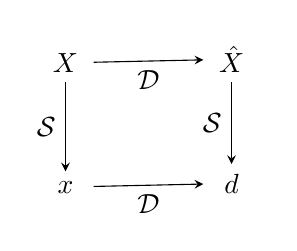
\begin{tikzpicture}
  \matrix (m) [matrix of math nodes,row sep=3em,column sep=4em,minimum width=2em]
  {
     X & \hat{X} \\
     x & d \\};
  \path[-stealth]
    (m-1-1) edge node [left] {$\mathcal{S}$} (m-2-1)
            edge node [below] {$\mathcal{D}$} (m-1-2)
    (m-1-2) edge node [left] {$\mathcal{S}$} (m-2-2)        
    (m-2-1) edge node [below] {$\mathcal{D}$} (m-2-2);
\end{tikzpicture}
\end{center}


\end{document}